\pdfoutput=1

\documentclass[conference,10pt]{IEEEtran} 

\IEEEoverridecommandlockouts

%\usepackage{draftwatermark}
%\SetWatermarkText{Draft}
\usepackage{balance}
\setcounter{tocdepth}{3}
\usepackage{cite}
\usepackage[numbers]{natbib}

\usepackage{graphicx}
\usepackage{algorithm}
\usepackage{algorithmic}
\usepackage{caption}
\usepackage{enumitem}
\usepackage[skins]{tcolorbox}
\usepackage{dblfloatfix}  
\usepackage{colortbl}
\usepackage{arydshln}
\usepackage{times}
\usepackage{rotating}
\usepackage{makecell}
\usepackage{tabularx}
\usepackage{booktabs}
\usepackage{wrapfig}
\usepackage{tikz}
\usetikzlibrary{angles}
\usepackage{makecell}
\usepackage{tabu}
\usepackage{multirow}
\usepackage{hyperref}
\usepackage{framed} 
\usepackage{newtxtext,newtxmath,amsmath}
\usepackage{cleveref}

\usepackage[framemethod=tikz]{mdframed}
\usetikzlibrary{shadows}
\usepackage{graphics}

\date{September 2020}

\begin{document}

\title{Layer-wise Adaptive Learning Rates Training}


\author{\IEEEauthorblockN{Noah Lozevski}
\IEEEauthorblockA{NC State University\\Raleigh, USA\\nlozevs@ncsu.edu}
\and
\IEEEauthorblockN{Huy Tu}
\IEEEauthorblockA{NC State University\\Raleigh, USA\\hqtu@ncsu.edu}
\and
\IEEEauthorblockN{Xianyang Wang}
\IEEEauthorblockA{NC State University\\Raleigh, USA\\xwang232@ncsu.edu}
}

\IEEEaftertitletext{\vspace{-2\baselineskip}}

\markboth{IEEE Conference on Machine Learning}%
{Tu \MakeLowercase{\textit{et al.}}: Large Batch Training of Convolutional Networks
for IEEE Journals}

\maketitle
\thispagestyle{plain}
\pagestyle{plain}
\IEEEpeerreviewmaketitle



\begin{abstract}
There is a direct relationship between a machine learning model's number of parameters and potential training time. This poses a large problem, as the first step taken to improve existing models is typically to increase the number of inputs/parameters. It is believed that these extra variables allow neural networks (NN) to better capture the latent data of the physical phenomena being studied. In the case of artificial neural networks, this is usually done by adding extra hidden layers or by increasing the resolution of the input. Breakthroughs in raw computational power have allowed many modern NN's to grow to a previously insurmountable size, some even containing 340 million parameters (XLNet). Even with the fastest GPU's available, this process still takes time and is a major hindrance in the research process. This high upfront cost (reaching over \$500,000 occasionally) has thus driven further research into optimizing the training process, rather than trying to develop faster hardware.

Most of the improvements in the effectiveness of the training process can be attributed to the advancement of stochastic gradient descent (SGD). These improved algorithms incorporate more information than just the gradient of the cost function, such as the first or second moments. Normalization techniques to account for training data variance also has been integrated, such as in the popular LARS, LAMB, or NVLAMB algorithms. These algorithms have allowed larger batch sizes (with similar test performance) at a fraction of the training time. Although the aforementioned algorithms derived from LARS have typically been focused on performance improvements in large-scale NN's, this paper aims to investigate their effectiveness in more challenging scenarios including but not limited to low training data situations, few-shot learning, and fine-tuning of transformer-based NLP models.
\end{abstract}

\begin{IEEEkeywords}
LARS, LAMB, SGD, Optimization
\end{IEEEkeywords}

\section{Introduction}
\label{sec:intro}
Deep neural networks typically have a large upfront cost associated with computational power and training dataset size. Even with modern training optimization algorithms such as Stochastic Gradient Descent~\cite{SGD}, training cost poses the biggest obstacle to achieving higher test accuracy. The advent GPU-based parallel processing has contributed the most to surpassing this obstacle, allowing previously impractical networks to become possible. For instance, training state-of-the-art NN's like BERT~\cite{bert} and ResNet-50~\cite{resnet} were able to be done in 3 days and 29 hours, respectively, as opposed to the original training time of several weeks. This feat was not possible even with the largest scale server processors before the beginning of this decade. 

Recent research in lowering training cost has been focused on optimizing the actual mathematical calculations during the process. Methods to make minor improvements include choosing optimal hyperparameters like the learning rate, automated perceptron pruning/dropout\cite{autopercept}, and by applying some form of gradient normalization. More complicated adaptive approaches attempt to better understand the direction of negative gradient to achieve more effective steps, typically using moving averages of the first and second moments. Popular optimizers like Adam and AdamW incorporate this adaptive approach and have shown substantial improvements over its predecessors\cite{Loshchilov2017FixingWD}. More advanced algorithms such as Layer-wise Adaptive Moments opti-mizer for Batch training (LAMB~\cite{You2020Large}) and Layer-wise Adaptive
Rate Scaling (LARS~\cite{qian2020impact, ginsburg2018large}) take this mentality several steps further and apply layer-wise adaptive gradient pre/normalization. You et al. showed that these approaches improve the initial loss decrease and allow for larger batch-size and distributed training while achieving comparable results (e.g. reducing BERT training time from three days to 76 minutes).  

However, the Machine Learning practitioners have been skeptical of these improvements and have not investigated or applied these layer-wise optimizers in their domains. This paper shall investigate, compare, and implement these innovative optimization techniques in relation to deep NN's in the Natural Language Processing (NLP), Computer Vision (CV) and Speech Processing domains. Specifically, the scope of the paper is focusing on the medium and smaller scale of the models (with median of 13 million parameters) in comparison to state of the art paper that testing the optimizers effectiveness on BERT ($\sim$110 million parameters). 


\begin{table}[t]
\centering
\caption{Overview of the studies: types of the explored tasks with corresponding models and optimizers}
\label{tab:LargeBatch}
\begin{tabular}{ccc} 
 \toprule
\textbf{Domain Task} & \textbf{Models} & \textbf{\# of Parameters} \\
 \midrule
  Image Classification & CNN \cite{CNN} & $\sim$440,000 \\
  QA System & DrQA \cite{DrQA} & $\sim$13,000,000 \\ 
  Speech to Text System & Deep Speech 2 \cite{deepspeech} &  $\sim$15,000,000\\
  \bottomrule
\end{tabular}

\vspace{10pt}

\begin{tabular}{cccc} 
 \toprule
 &  \multicolumn{2}{c}{\textbf{Optimizers}} & \\
 \midrule
 SGD \cite{SGD} & LARS \cite{ginsburg2018large} & Adam \cite{adam}  &  LAMB \cite{You2020Large} \\
  \bottomrule
\end{tabular}
\end{table}

The study cases include: 

\begin{itemize}
    \item Image classification is a process of labeling and categorizing pictures. For most image classification tasks, convolutional neural networks are the most effective at achieving high accuracy with a moderate number of perceptron connections. However, with recurrent convolutional and pooling layers, these networks can become very deep (large number of parameters) relatively quickly\cite{CNN}. Many issues arise with standard back-propagation techniques of these deep CNN's, putting a large burden on the effectiveness of the optimizer chosen to train the model. Even after thousands of iterations and epochs, some optimizers still fail converge to optimal weights\cite{Sun2019OptimizationFD} with used on models with high numbers of layers. 
    % We expect that the layer-wise approach taken by the LAMB or LARS optimizers will thus improve training time of these types deep networks significantly, as they should be able to better incorporate information from the individual layer gradients. This decrease in training time should be seen as a faster decrease in the loss function value while still maintaining relatively similar accuracy on the test/validation set.
    
    \item Another common application of machine learning is the use of NN's for question answering (QA) system, which belongs to the category of information retrieval. These systems consist of three parts: question classification, information retrieval, and answer extraction. Since these models  must be able to respond with a large vocabulary and are very dynamic in nature, they usually suffer from extremely large training times. The overall architecture of the model we will test will include a LSTM network with attention, which is the standard model used in production. 
    
    %We believe that the application of layer-wise adaptive scaling and pre-normalization will improve the initial loss decrease and allow for larger batch-size/distributed training.\\
    \item The final type of machine learning model tested in this paper will be a speech to text system. This involves transforming raw audio signals into human-readable text. Consumer products such as the Amazon Alexa, Siri from Apple, the Google Assistant all utilize the most cutting-edge speech-to-text models. These models are usually multimodal including acoustic, pronunciation, and language models. Each part can utilize a deep NN to train separately and that makes speech recognition algorithms very computationally expensive and incorporate extremely large numbers of trainable parameters. 
    
    %We expect that optimizer's like LAMB/LARS could help reduce this computational cost of training when used on modern speech-to-text architecture such as the LAS model\cite{LAS}.

\end{itemize}

According to You et al. \cite{ginsburg2018large, You2020Large} work, we also expect that the layer-wise approach, LAMB or LARS optimizers, will thus improve training time of deep networks for these application domains by adaptively learn the initial losses. It can better incorporate information from the individual layer gradients. This decrease in training time should be seen as a faster decrease in the loss function value while still maintaining relatively similar performance.


In summary, the contributions of our study include:
\begin{enumerate}
    \item Validate the previous work results that this paper based on \cite{ginsburg2018large,You2020Large}.
    \item Explore more study cases (NLP, CV, and Speech) and model sizes (median of 13 million parameters than the original work did (only ResNet50 \cite{resnet} and BERT \cite{bert}). 
    \item Testing the effectiveness of layer-wise optimization techniques on smaller batch sizes training (8 as the smallest for Speech and 64 for NLP)  as the You et al. tested on large batch sizes of {4k and >8k}.
\end{enumerate}




%but are based on some forms of a Hidden Markov Model (HMM) \cite{HMM}. Preprocessing of the input data is usually done by dividing the speech signal into segmented chunks and applying signal processing transforms (i.e. Fast Fourier Transform)\cite{FFT}. This makes speech recognition algorithms very computationally expensive and incorporate extremely large numbers of trainable parameters. We expect that optimizer's like LAMB/LARS could help reduce this computational cost of training when used on modern speech-to-text architecture such as the LAS model\cite{LAS}.







% \begin{table}[!t]
% \vspace{-15pt}
% \scriptsize
% \vspace{7pt}
% \caption{Plan of project work.}\label{tbl:planofwork}
% \vspace{-15pt}
% \begin{center}
% \begin{tabular}{ l|c|l}
%   \multicolumn{1}{c|}{Standard} &
%  \multicolumn{1}{c|}{Date} &
%  \multicolumn{1}{c}{Responsibilities}\\
%  %& & \\
% \hline
% & & We will research necessary papers and  \\
%  Literature Review & 9/07 - 9/25 &  contribute information to address how the  \\
%  & &  problem relates to the group's interests. \\\hline
% & & Each of us will propose appropriate \\
% Experiment Setup & 	09/25 - 10/02 & application, setting, and dataset for this\\
% & &  project's direction.\\\hline
% & & We will delegate coding parts based off of \\
% Implementation & 10/02 - 10/16  & each individual's strength (e.g. each optimizer \\
% & & per individual group member) \\\hline
% & & We will share the exploration of applicable \\
% Mathematical and & 10/16 - 10/30 &  theories (e.g. LARS \& LAMB) while \\ 
% Result Analysis & &	  evaluate the results deeply in regards to  \\
% & & the problem's context\\\hline
% & & Each of us will help report background \\
% Documentation & 10/30 - 11/13 &  theories, outcomes, discussion, and possible\\
% & &  future directions. \\


% \end{tabular}
% \end{center}
% \vspace{-15pt}
% \end{table}
% 1 pg
\section{Background}
\label{sec:background}
\subsection{Optimizers}


Training a large deep neural network is very computationally expensive. The training of CNN and LSTM are typically optimized using Stochastic Gradient (SG) and Adam based methods.  At each step $t$ a minibatch of $B$ samples $x_i$
is selected from the training set. Increasing the capacity of the mini-batch permits scaling to more nodes without reducing
the workload on each unit. At the same time, training with a large batch has been observed to be difficult \cite{Krizhevsky}. Krizhevsky (2014) suggested the following rules for training with large batches: when you increase
the batch $B$ by $k$, you should also increase the learning rate by $k$ in order to do reduce $k$ steps.  It was observed that linear scaling works much better for networks with Batch
Normalization (e.g. Codreanu et al. (2017)). For example Chen et al. (2016) trained the Inception
model with batch $B=6400$, and Li (2017) trained Resnet-152 for $B=5K$. Two main problems of such large batch training include: 

\begin{itemize}
    \item The instability of training with high learning rates (LR). Goyal et al. suggested the LR warm-up policy to start with a small LR and switch to the regular LR after a few epochs. They were able to combine that with linear scaling to train Resnet-50 with batch $B=8K$ with loss in accuracy. 
    
    \item There is a lack of generalization ability, according to Keskar et al. \cite{Keskar}, the large-batch methods seem to converge to sharp minimizers of the training function. Adaptive learning rates have gathered interests to solve this problem and also to help reduce the hand-tuning of hyperparameters \cite{adaplr}.  
\end{itemize}




You et al. (2017) proposed a new training algorithm of LARS to solve this problem. The intuition is to adapt the learning rate on each layers that is SG based. Using the LARS algorithm, the Alexnet can be trained with a batch size of 8k and Resnet-50 can be trained with a batch size of 32k without loss in accuracy. However, LARS performs poorly for attention models like BERT. 


Inspired by LARS, You et al. (2019) developed a new optimization algorithm Layer-wise Adaptive Moments optimizer for Batch training (LAMB) especially for large batch size training. The adaptivity of LAMB are different from LARS in two parts: (1) parameter normalization based on the square root of the second moment in Adam; and (2) layer-wise adaptive normalization. The author reported that by training the BERT language model with LAMB optimizer can drastically reduce the training time from 3 days to 76 minutes without the reduction of performance.

\subsection{Case Studies}


\subsubsection{Computer Vision - Image Classification}

\begin{figure}[!t]
    \centering
    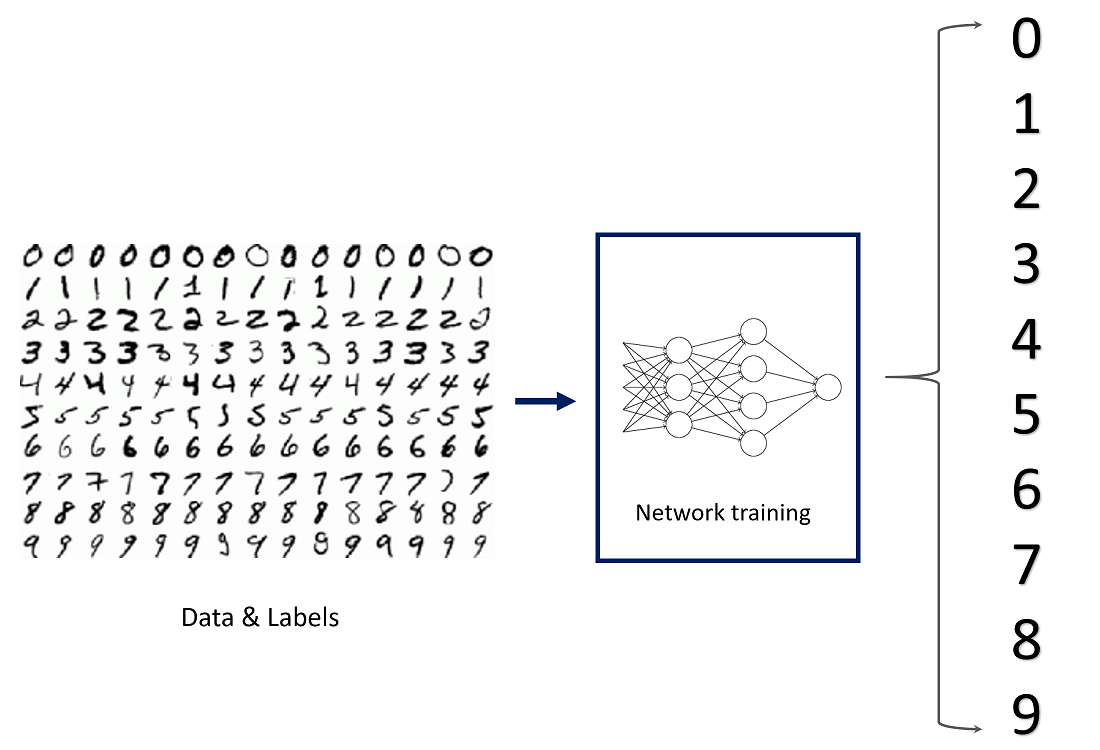
\includegraphics[width=\linewidth, height=7cm]{img/mnist.png}
    \caption{An overview of the image classification in an example of handwritten digits classification.}
    \label{fig:DrQA_overview}
    \vspace{-10pt}
\end{figure}

One of the classical task over the past 10 years in the machine learning community is image classification with the proposal of many new models and the creation of benchmark datasets. For instance, this study focuses on handwritten digit recognition or optimal character recognition (OCR) of MNIST database by LeCun et al. \cite{LeCun}. Before the advancement of GPU is 2012, traditional machine learning approaches have served as the baseline for this OCR task tested on MNIST database including K-Nearest Neighbor, ensemble-based classifiers, and Support Vector Machine. After 2012, Convolutional Neural Network (CNN) emerged and served as the new baseline for this benchmark dataset in OCR task.
The traditional CNN model, where the earliest date can be traced back
to the 1986 Back Propagation algorithm \cite{BP}. Then in 1989 LeCun used it
in multi-layer neural networks \cite{1989Lecun} which is then extended to LeNet-5 model in 1998. The CNN's architecture allows take advantage of the
two dimensional structure of the input data in order to capture a deeper understanding of these images.



\begin{figure}[!t]
    \centering
    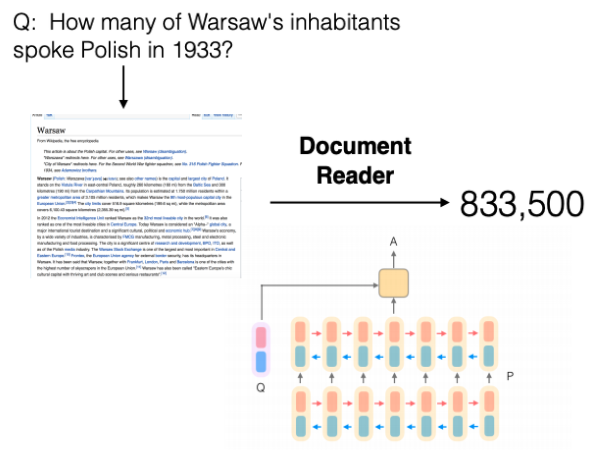
\includegraphics[width=\linewidth]{img/QA.png}
    \caption{An overview of the question answering system DrQA \cite{DrQA}.}
    \label{fig:DrQA_overview}
    \vspace{-10pt}
\end{figure}



\subsubsection{NLP - Question Answering System}

The NLP specific task we picked for this paper is open-domain QA originally rooted in finding answers in collections of unstructured documents following the annual Text REtrieval Conference competitions (TREC\footnote{https://trec.nist.gov/data/qamain.html}). First, the development of Knowledge Base (KBs) have pushed a lot of resources creation like WebQuestion \cite{webquestion} and SimpleQuestion \cite{simplequestion} or automated extracted KBs like NELL \cite{KBNELL}. Yet, KBs have inherent nature that limiting these work including fixed schemas and incompleteness. Therefore, researchers have to return to the original setting of answering from raw text. 



Secondly, it is a distinct subfield of machine comprehension of text. With the advancement of deep learning architectures like attention-based and memory-augmented neural network \cite{attention} \cite{attention2} \cite{attention3}, researchers have made considerable progress.  The adopted QA system  for this study shall utilize these new methods.


Other previous researchers also considered other resources of semi-structured knowledge such as infoboxes, article structure, category structure, and definitions \cite{Ryu}. Yet, this QA system only consider the comprehension of text only, or relying on a single resource.
    
    






Therefore, this study focused on the inspired Document retriever Question Answering (DrQA) similar to Figure \ref{fig:DrQA_overview}. As the name suggested, it composed of (1) Document Retriever and (2) Document Reader where for this study's purpose of model's optimization will not consider part 1 of the system and solely focus on part 2. Specifically, for Document
Reader, a multi-layer recurrent neural network
machine comprehension model trained to detect
answer spans in those defined context.




\subsubsection{Speech - Speech-to-Text}

Another study case which is essential to a lot of virtual or smart home assistant is speech recognition. As previously mentioned, our goal is to output reasonable transcription according to the audio segment. A general system is illustrated in the Figure \ref{fig:speech2text}. For more than 20 years ago, feed-forward
neural network acoustic models were explored \cite{acoustic} \cite{acoustic2}.  More recently DNNs have become a fixture in the ASR pipeline with almost all
state of the art speech work containing some form of deep neural network \cite{DNN}. From CNN successes with acoustic models \cite{CNNacoustics}, recurrent
neural networks (typically LSTMs), are beginning to be adapted in state-of-the art recognizers \cite{recognizers} that thrive on convolutional layers for the feature extraction \cite{featextr}. World-wide recognized level of such models include Deep Speech by Baidu \cite{deepspeech} and Listen Attend Spell (LAS) by Google \cite{LAS}. We adapted a model that is similar to Deep Speech 2 architecture \cite{deepspeech} which utilized enhanced numerical optimization through SortaGrad and Batch normalization, RNNs evaluation with larger strides with bigram outputs, and searching through bidirectional and unidirectional models.


\begin{figure}[!t]
    \centering
    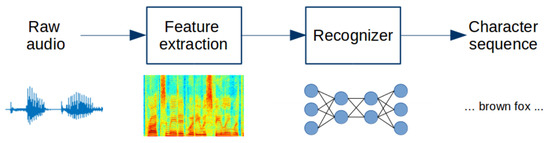
\includegraphics[width=\linewidth]{img/speech2text.jpg}
    \caption{An overview of Speech 2 Text end to end system}
    \label{fig:speech2text}
\end{figure}

For learning the audio features, the author employed the Residual CNN which was first introduced by He et al. \cite{resnet} to learn the skip connections (i.e. residual connections) for faster and more generalizable audio features. Specifically, these networks shall have a smoother loss surface when visualizing to make it easier to navigate the landscape and find a lower and more generalizable loss minima.  For leveraging the previously learned features, the bidirectional recurrent neural network (RNN) is employed which first introduced by for being good at sequence modeling problem. Specifically, RNN helps learn the context of frame before each step and the frame after it as well. The author employed Gated Recurrent Unit (GRU's) variant which is simpler than traditional Long Short Term Memory (LSTM) in (1) avoiding the usage of memory unit that LSTM does and (2)  LSTMs have computations  separating the update gate and forget gate which lead to the architecture more complex and less efficient to GRU. 



% 1-2 pgs
% Need section for related work, and a separate section for
% the different study cases (why do we study them?)


\section{Methodology}
\label{sec:method}
\subsection{Optimizers}

A neural network learns to map a set of inputs, \textbf{\textit{X}}, to a corresponding set of outputs, \textbf{\textit{Y}}, while given a subset of correct mappings (training data), $\textbf{\textit{D}}$, where $\textbf{\textit{D}} \subset \textbf{\textit{X}}$, and
% \begin{equation}
%   \begin{aligned}
%     D \subset X
%   \end{aligned}
% \end{equation}
% \begin{equation}
%   \begin{gathered}
%     D = \{(x_i,y_i),...,(x_k,y_k)\}
%   \end{gathered}
% \end{equation}
\begin{center}
$\textbf{\textit{D}} = \{(x_i,y_i),...,(x_k,y_k)\},$
\end{center}
where $(x_i,y_i)$ are individual samples. The network takes the input samples and performs a number of sequential operations to create output estimates, denoted by $\hat y_i$. During the training phase of a neural network, the objective function to be minimized is the derived cost function, $J$, which is remapped to create the loss function $L$, which is dependent on the weights/parameters of the network, $w_i$, as well as $x_i$ (the inputs), $\hat y_i$ (the outputs), and $y_i$ (the correct labels). Thus, training of a neural network can be represented as the optimization problem:

\begin{center}
$\min\limits_{x_i \in X} L(w_i,x_i,y_i,\hat y_i)$
\end{center}

Since the objective function shown above is typically non-convex and can have many pseudo-optimal solutions, direct solutions of the cost function are not feasible. Instead, gradient descent algorithms are used to find these locally minimizing set of parameters using the training data and the corresponding cost/loss function.

In any gradient descent algorithm, a random (or predetermined) initial point, $x_0$, is chosen and then each subsequent value $x_{t+1}$ is determined with the following general updating rule:
\begin{center}
$x_{t+1} = x_t - \eta_t \nabla L_t(w_i,x_i,y_i,\hat y_i) $
\end{center} 
where $\eta_t$ is step length (learning rate), and $\nabla L_t$ is gradient at the current time step. Different algorithms incorporate more variables and calculations into this update step, and/or can add more normalization steps in between updates.

\subsubsection{SGD Algorithm}

The SGD algorithm is one of the most common (and basic) gradient descent algorithms used in the neural network training. The adapted algorithm for mini-batches is as follows:
\vspace{14pt}
\begin{minipage}[b]{.48\textwidth}
\begin{algorithm}[H]\small
	\caption{$Mini-batch\:SGD$ \cite{SGD}}
	\label{alg:SGD}
	\begin{algorithmic}
		\STATE {\bfseries Input:} $x_i \in \mathbb{R}^d$, learning rate $\{\eta_t\}_{t=1}^T$, mini-batch size $B$, $\epsilon>0$
		\vspace{2pt}
		\FOR{$t=1$ {\bfseries to} $T$}
		\vspace{2pt}
		\STATE $G^{(t)}\coloneqq 0$
		\vspace{2pt}
		\FOR{$k=1,...,B$}
		    \vspace{2pt}
		    \STATE Randomly sample point $(\tilde x_k,\tilde y_k)$ from \textbf{\textit{D}}
		    \vspace{2pt}
		    \STATE Compute $\hat y_k$ from current network weights, $w_t$
		    \vspace{2pt}
		    \STATE $G^{(t)}\leftarrow G_k^{(t)} + \frac{1}{B}\nabla L(w_t,\tilde x_{k},\tilde y_k,\hat y_k)$
		    \vspace{4pt}
		\ENDFOR
		\vspace{2pt}
		\STATE $w_{t+1} = w_{t} + \eta_t (G^{(t)} + \epsilon)$
		\vspace{4pt}
		\ENDFOR
	\end{algorithmic}
\end{algorithm}
\end{minipage}\hfill
\vspace{-8pt}

In summary, the mini-batch SGD algorithm states that for every mini-batch (from $1,...,\textit{T}$), the gradient of the loss function will be summed and averaged for each individual sample, $(\tilde x_k,\tilde y_k)$, and the resulting update value $G^{(t)}$ will be used to update the current network weights, $w_i$. The advantage behind performing mini-batches as opposed to weight updates after individual samples is for two reasons:
\vspace{4pt}
\begin{enumerate}
    \item Averaging the gradient across samples has been shown to lower the chances of over-fitting[]
    \item Weight-updates can be performed in a parallel / asynchronous setting, where work can be distributed across individual processors and summed at the end
\end{enumerate}
\vspace{3pt}

Mini-batch SGD has been shown to easily converge many moderately sized neural networks, but fails when the network becomes large or when there is large variance sample to sample.
\subsubsection{LARS optimizer}

The LARS optimizer (short for Layer-wise Adaptive Rate Scaling), developed and outlined by \_ in \cite{ginsburg2018large}, improves upon the previous SGD algorithm by scaling learning rate across individual layers. You et al. found that the ratio of $||w_t||$ ($l_2$ norm of the current weights) to $||g_t||$ (the gradient at the current time step) varied tremendously from the initial to final layers. They propose that scaling the learning rate $\eta_t$ by a second parameter called the "trust" or "lars" coefficient and by the ratio $\frac{||w_t||}{||\nabla L(w_t^l)||}$, training should substantially improve for deep neural networks. They proved this was the case for the ResNet-50 model even when trained with extremely large batch sizes (greater than 32k)\cite{ginsburg2018large}. An outline of the algorithm in the case of SGD with LARS and momentum is as follows:
\begin{minipage}[b]{.48\textwidth}
\begin{algorithm}[H]\small
	\caption{SGD with LARS and momentum \cite{ginsburg2018large}}
	\label{alg:lars}
	\begin{algorithmic}
	    \vspace{3pt}
		\STATE {\bfseries Input:} $x_i \in \mathbb{R}^d$, learning rate $\{\gamma_t\}_{t=1}^T$, $0 < \beta_{1} < 1$ (momentum scaling), LARS coefficient $\eta <1$
		\vspace{3pt}
		\STATE $m_{0} = 0$ (initial momentum term to zero)
		\FOR{$t=1$ {\bfseries to} $T$}
		\vspace{2pt}
		\STATE Randomly sample point $(\tilde x_k,\tilde y_k)$ from \textbf{\textit{D}}
% 		\STATE Draw b samples $S_t$ from $\mathbb{P}$
        \vspace{3pt}
		\STATE $\hat y_k$ (from current network weights, $w_t$)
		\vspace{2pt}
        \STATE $\nabla L(w_t^l,\tilde x_k,\tilde y_k,\hat y_k)$ (gradient at each layer)
        % = \frac{1}{|\mathcal{S}_t|} \sum_{s_t \in \mathcal{S}_t}\nabla \ell(x_t, s_t)$
        \vspace{3pt}
        \STATE $\lambda^l \gets \frac{||w_t^l||}{||\nabla L(w_t^l)||}$ (local LR)
        \vspace{3pt}
        
        \STATE $v_{t} = \beta v_{t-1} + \gamma_t\eta(1 - \beta)\lambda^l\nabla L(w_t^l)$ (momentum calculation)
% 		\STATE $v_{t+1}^l = \eta_t  ||w_t^{(i)}||\frac{m_t^{(i)}}{\|m_t^{(i)}\|} $ for all $i \in [h]$
        \vspace{3pt}
		\STATE $w_{t+1} = w_{t} - v_t$ (update weights)
		\vspace{3pt}
		\ENDFOR
	\end{algorithmic}
\end{algorithm}
\end{minipage}\hfill%
% \begin{algorithm}[htb!]%[t]
% \begin{algorithmic}
% \STATE {\bf Parameters:} base LR $\gamma_0$, momentum $m$, weight decay $\beta$, LARS coefficient $\eta$, number of steps $T$
% \STATE {\bf Init:} $t = 0, v = 0$. Init weight $w_0^l$ for each layer $l$
% \WHILE {$t < T$ for each layer $l$} 
%         \STATE $g_t^l \gets \nabla L(w_t^l)$   (obtain a stochastic gradient for the current mini-batch)
%         \STATE $\gamma_t \gets \gamma_0 * \left(1 - \frac{t}{T}\right)^2$ (compute the global learning rate)
%         \STATE $\lambda^l \gets \frac{||w_t^l||}{||g_t^l|| + \beta ||w_t^l||}$       (compute the local LR  $\lambda^l$)
%         \STATE $v_{t+1}^l \gets mv_t^l + \gamma_{t+1} * \lambda^l * (g_t^l + \beta w_t^l)$     (update the momentum)
%         \STATE $w_{t+1}^l \gets w_t^l - v_{t+1}^l$ (update the 
%         weights)
% \ENDWHILE
% \end{algorithmic}
%  \caption{Mini-batch SGD with LARS. Example with momentum\label{algo:lars}}
% \end{algorithm}

It is important to note that there are two key differences between this implementation and traditional SGD with momentum:
\begin{enumerate}
    \item The learning rate is now parameterized by the layer number, $l$
    \item The calculation of the trust coefficient, $\lambda^l$, is scaled by the LARS coefficient, $\eta$, to apply different magnitudes of LR scaling for each layer
\end{enumerate}
\vspace{4pt}

It can be deduced that dividing by the $l_2$ norms of the loss function and weight vector is effectively normalizing the magnitude of the update step. In practice, this means that only the direction of the gradient is taken into consideration for each update step. It is assumed that this layer-wise normalization allow for deep networks to be trained for higher numbers of iterations with a less likelihood of over-fitting. When applied to the mini-batch case, gradient updates are performed in the same manner, where the gradient updates at each mini-batch are averaged to make a singular update. 

\subsubsection{ADAM optimizer}
Although LARS makes many improvements to traditional SGD algorithms, it still does not incorporate higher-order terms that could benefit each update step. The ADAM optimizer, created by \_ in \cite{adam}, enhances regular gradient descent algorithms through the addition of two terms and two hyperparameters:
% It introduces exponential moving average on the first and second order of the gradient:
\vspace{-10pt}
\begin{align*}
m_{t} = \beta_{1}m_{t-1}+(1-\beta_{1})g_{t} \\
v_{t} = \beta_{2}v_{t-1}+(1-\beta_{2})g_{t}^2
\end{align*}

The first and second term, $m_{t}$, $v_t$, represent the exponential moving average of the first and second moment of the gradient of the loss function, $g_t$, respectively. The two hyper parameters, $\beta_1$ and $\beta_2$ represent the weighting of the previous and current values. After calculating these two values, there is also a bias correction step:
\begin{align*}
\hat{m}_{t}=\frac{m_t}{1-\beta_1^t} \\
\hat{v}_{t}=\frac{v_t}{1-\beta_2^t}
\end{align*}
\vspace{-10pt}

The addition of these two terms comes from the calculation of the expected value of each moment, which is corrected by dividing the current moment by $(1 - \beta_i^t)$, where t is the current step number. This operation makes $m_t$ and $v_t$ \textit{unbiased estimators} of the first and second moment of the gradient. The algorithm is as follows:
\begin{minipage}[b]{.48\textwidth}
\begin{algorithm}[H]\small
	\caption{ADAM \cite{adam}}
	\label{alg:adam}
	\begin{algorithmic}
		\STATE {\bfseries Input:} $x_i \in \mathbb{R}^d$, learning rate $\{\eta_t\}_{t=1}^T$, parameter $\beta_{1},\beta_{2} \in [0,1)$,  $\epsilon > 0$
		\STATE Initialize $m_{0} = 0, v_{0} = 0$
		\FOR{$t=1$ {\bfseries to} $T$}
		\vspace{2pt}
		\STATE Randomly sample point $(\tilde x_k,\tilde y_k)$ from \textbf{\textit{D}}
		\vspace{2pt}
		\STATE Compute $\hat y_k$ from current network weights, $w_t$
		\vspace{2pt}
		\STATE $g_{t} = \nabla L(w_t,\tilde x_{k},\tilde y_k,\hat y_k)$
		\vspace{2pt}
        \STATE $m_{t} = \beta_{1}m_{t-1}+(1-\beta_{1})g_{t}$
        \vspace{2pt}
        \STATE $v_{t} = \beta_{2}v_{t-1}+(1-\beta_{2})g_{t}^2$
        \vspace{2pt}
        \STATE $\hat{m}_{t}={m_t}/(1-\beta_1^t)$
        \vspace{2pt}
        \STATE $\hat{v}_{t}={v_t}/(1-\beta_2^t)$
        \vspace{2pt}
        \STATE $w_{t+1} = w_{t}-\eta_t\frac{\hat{m}_t}{\hat{v}_t+\epsilon}$
        \vspace{2pt}
		\ENDFOR
	\end{algorithmic}
\end{algorithm}
\end{minipage}\hfill%

\subsubsection{LAMB optimizer}

The LAMB algorithm, developed by \_ in \cite{You2020Large} uses ADAM as the base algorithm, by applies the same layer-wise normalization that LARS implements. More specifically, it makes the following adjustments:
\begin{enumerate}
    \item Using the square root of second moment for normalization
    \item Adopting layer-wise normalization
\end{enumerate}
\begin{minipage}[b]{.5\textwidth}
\begin{algorithm}[H]\small
	\caption{$LAMB$ \cite{You2020Large}}
	\label{alg:lamb}
	\begin{algorithmic}
		\STATE {\bf Input:} $x_1 \in \mathbb{R}^d$, learning rate $\{\eta_t\}_{t=1}^T$,  parameters $0 < \beta_{1}, \beta_2 < 1$, scaling function $\phi$, $\epsilon > 0$
		\STATE Set $m_{0} = 0$, $v_{0} = 0$
		\FOR{$t=1$ {\bf to} $T$}
		\STATE Draw b samples $S_t$ from $\mathbb{P}$.
        \STATE Compute $g_t = \frac{1}{|\mathcal{S}_t|} \sum_{s_t \in \mathcal{S}_t}\nabla \ell(x_t, s_t)$.
		\STATE  $m_{t} = \beta_{1} m_{t-1} + (1 - \beta_{1}) g_{t}$ 
		\STATE  $v_{t} = \beta_{2} v_{t-1} + (1 - \beta_{2}) g_{t}^2$
		\STATE $m_t = m_t/(1 - {\beta}_1^t)$ 
        \STATE $v_t = v_t/(1 - {\beta}_2^t)$
		\STATE Compute ratio $r_t = \frac{m_t}{\sqrt{v_t} + \epsilon}$
		\STATE $x_{t+1}^{(i)} = x_{t}^{(i)} - \eta_t \frac{\phi(\|x_t^{(i)}\|)}{\|r_t^{(i)} + \lambda x_t^{(i)}\|} (r_t^{(i)} + \lambda x_t^{(i)})$
		\ENDFOR
	\end{algorithmic}
\end{algorithm}
\end{minipage}

\subsection{Study Cases' Models}




\subsubsection{Image Classification}

\begin{enumerate}[start=1,label={\bfseries\arabic*:}]
    \item A set of convolution layer and pooling layer to compress the image
    \item Another set of convolution layer and pooling layer to further compress the data
    \item Two fully connected layers after flattens the data to do the neural network training.
    \end{enumerate}
    
%The first part of the network is a straightforward CNN model and it uses Relu as activation function. It consists of two consecutive convolution layer and pooling layer in order to capture the potential features of the images. The second part of the network flattens the condensed image and then uses two fully connected layer to do the classification.

The cost function is calculated by negative log likelihood loss:
\begin{align*}
    J(y) = -log(y) 
\end{align*}

Note there is only one term in the loss function per data, which is the negative log likelihood of the predicted value of the true label. This negative loss likelihood function works better when the neural network model has a high confidence at the correct class. When training in batch, the cost function per batch is the sum of the individual negative log likelihood costs.

\subsubsection{QA System}


The model employed for QA understanding system here is called Document retriever Question Answering (DrQA) as illustrated in Figure~\ref{fig:DrQA}.  Starting from the top:
\begin{enumerate}[start=1,label={\bfseries\arabic*:}]
    \item According to Lee et al. \cite{Lee}, the questions and context can be aligned to build respective embedding of: 
    \begin{center} $f_{align} = \sum_j \alpha_{i, j} E(q_j)$. \end{center}
    
    Where $\alpha$ is single dense layer with relu non-linearity and $E()$ represents the glove embeddings. This layer help initialize what portion of the context is more important or relevant with respect to the question.
    
    \item In order to understand the representation of these glove and aligned paragraphs, these are passed to stacked bi-LSTM \cite{biLSTM}. LSTM is expressed as: 
    \begin{center}
    $u_t = \sigma(W_u x_t + U_u h_{t-1} + b_u)$ \\
    $f_t = \sigma(W_f x_t + U_f h_{t-1} + b_f)$  \\
    $g_t = tanh(W_g x_t + U_g h_{t-1} + b_g)$  \\
    $o_t = \sigma(W_o x_t + U_o h_{t-1} + b_o)$  \\
    $c_t = f_t c_{t-1} + u_t g_t$ \\
    $h_t = o_t tanh(c_t)$
    \end{center}
    
    where $u, f, g, o$ are  respectively update/input, forget, cell, and output gates. $c_t$ is the cell at time $t$ and $\sigma(\cdot)$ is the sigmoid function. 
    
    \item Then the importance of each word in the question is calculated through Linear Attention layer as $b$ below with $w$ as a trainable weight vector:
    \begin{center} 
    $b_j = \frac{e^{w \cdot q_j}}{\sum_{j'}e^{w\cdot q_{j'}}}$
    \end{center}
    
    \item Finally, to predict the accurate answer's span tokens, there are two bilinear classifiers to respectively predict the probabilities of start and end tokens of the span: 
    \begin{center} 
    $P_{start}(i) \propto e^{p_iW_sq}$ \\
    $P_{end}(i) \propto e^{p_iW_eq}$
    \end{center}
    
    
\end{enumerate}


\begin{figure}[!t]
    \centering
    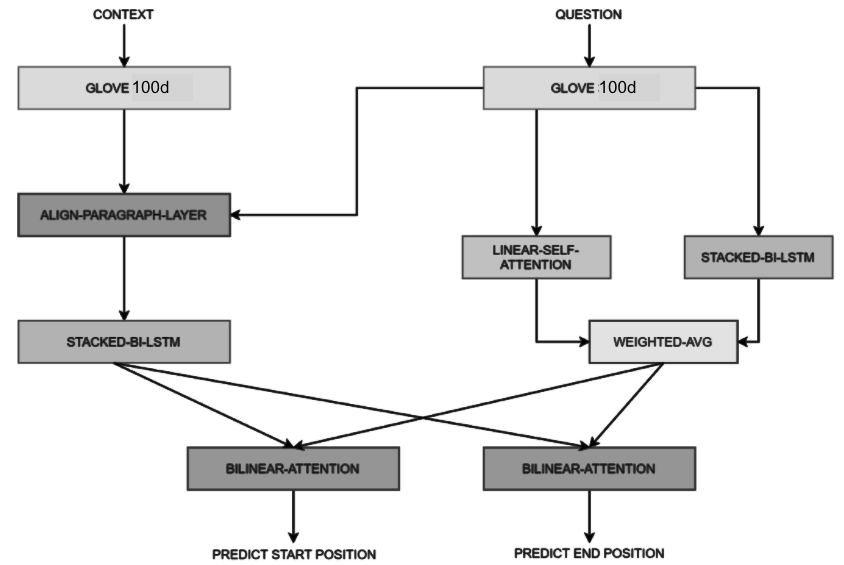
\includegraphics[width=\linewidth]{img/DrQA.png}
    \caption{Document Reader model architecture part of DrQA \cite{DrQA}}
    \label{fig:DrQA}
\end{figure}

% As the name suggested, the model included Document Retriever and Document Reader: 




\subsubsection{Speech to Text}

The model is a variant of the Deep Speech 2 model with the aid of Residual CNN (Res-CNN)

% Model is similar to Deep Speech 2, model, but first preprocesses the data into a spectrogram, then these are fed into 3 Residual CNN blocks to extract feature vectors of length 500 from the audio data, and a set of 3 bidirectional GRU-RNN layers to translate the extracted features into an intermediate output vector, which is fed into a fully connected layer, then a softmax, then a 28 long vector mapping of probabilities of corresponding letters or symbols.

\begin{figure*}[!t]
    \centering
    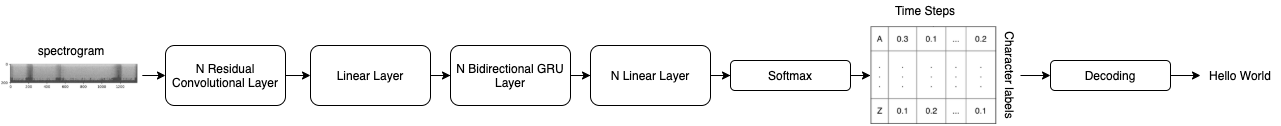
\includegraphics[width=\linewidth]{img/speech.png}
    \caption{A variant of Deep Speech 2 architecture that utilizes Res-CNN.}
    \label{fig:deepSpeech}
    \vspace{-10pt}
\end{figure*}

\begin{enumerate}[start=1,label={\bfseries\arabic*:}]
    \item Residual network consists of stacked ``residual units'' inspired by He et al. \cite{resnet} but with layer norm to learn the audio features expressed as:
    \begin{center}
    $x_{l + 1} = ReLU(h(x_l) + F(x_l, W_l))$ \\
    \end{center}
    
    \item A fully connected layer to compress the model representation before passing it over. 
    
    \item Bidirectional GRU-RNN \cite{biGRURNN} is then utilized to leverage the features to learn the representation of the audio's spectrogram frames before the current step and after it as well. 
    
    \begin{center}
    
    $u_t &= \sigma(W_u x_t + U_u h_{t-1} + b_u)$ \\
    $r_t &= \sigma(W_r x_t + U_r h_{t-1} + b_r)$ \\
    $\tilde{h}_t &= f(W_h x_t + r_t \circ U_h h_{t-1} + b_h)$ \\
    $h_t &= (1 - u_t) h_{t-1} + u_t \tilde{h}_t$

    \end{center}
    
    $u$ and $r$ represent the \emph{update} and \emph{reset} gates respectively. This is slightly different from the standard GRU in that the hidden state $h_{t-1}$ is multiplied by $U_h$ prior to scaling by the reset gate. This allows for all operations on $h_{t-1}$ to be computed in a single matrix multiplication. Moreover, Amodei et al. \cite{Amodei} found similar performance for $tanh$ and clipped-ReLU for nonlinear transformation so clipped-ReLU \cite{clippedReLU} is picked for simplicity and uniformity with the rest of the network.

    
    \item A final fully connected layer takes the inputs from the feature analysis and applies weights to predict the correct label.
    
    \item A Gaussian Error Linear Unit (GELU) activation layer as: 
    
    \begin{center}
    $GELU(x) = xP(X \leq x) = x \cdot \frac{1}{2} [1 + erf(\frac{x}{\sqrt{2}}]$
    \end{center}
    
    \item A linear layer to map the results to final probabilities for each mapping of corresponding letters or symbols. 
    
\end{enumerate}


% 1.5 pgs
% different section for each optimizer (SGD, lars, lamb, adam)
% for each section, go over initial background of how it was made, the math behind it
% for the lars/lamb show the difference between their baseline comparisons (so SGD/adam)



% \section{Experimental setup}
% \label{sec:experiments}
% 

\subsection{Image Classification Setup}

% Image Classification Task
%     Dataset
%     Architecture
%     Implementation Details (coding aspect, where it is in the repo, hyperparameters)
%     Evaluation
% Question Answering System Task
% Speech-to-Test Decoding Task




\subsubsection{Dataset}

In this paper we used EMNIST \cite{emnist} data set, which is a collection of handwritten characters and digits from NIST Special Database 19. The data is converted to 28 by 28 matrix so its format matches MNIST data set. There are six subsets in the EMNIST data set: ByClass, ByMerge, Balanced, Letters, Digits and MNIST. We chose the Letter subset because there are around 145k data in it, which will result in a decent running time without loss of information. In the Letter subset, there are 26 classes which corresponding to letter A to letter Z.
\begin{figure}[htp]
    \centering
    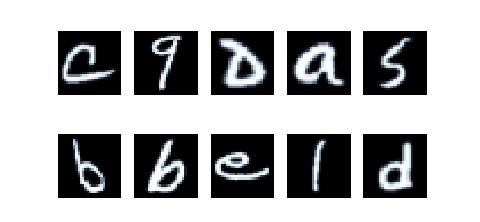
\includegraphics[width=8cm]{img/EMNIST.png}
    \caption{Data instances in EMNIST, which are handwritten 26 alphabetical characters.}
    \label{fig:EMNIST}
\end{figure}



\subsubsection{Evaluation}



The batch size for training is {512, 1024, 2048, 4096, 8192}, the test size is 2048. we keep track of the train loss, test accuracy and test loss for every epoch when using those different optimizers to train the model. For the optimizers, we keep track of the trust ratio and the weight norm of them.




\subsection{Question Answering System Setup}

\subsubsection{Dataset}

For our QA system task, the SQuAD dataset curated by Rajpurkar et al. \cite{squad} is employed. There are 80,000 instances for training and 30,000 instance for testing. For each instance, there are question, answers and the context that the question and answer are based on along with the boundary label of the answer. The task is to read the question in order to (1) retrieve the relevant context and (2) then locate the start and end position of the answer. Example of such an instance is shown in Table \ref{tbl:qasystem}. 

\begin{table}[!b]
\vspace{-5pt}
\scriptsize
\vspace{7pt}
\caption{QA System SQuAD examples. Noted \textit{label} indicating the span of the \textit{answer} inside the context for the corresponding question. }\label{tbl:qasystem}
\vspace{-10pt}
\begin{center}
\begin{tabular}{ l|c|c|l}
 \multicolumn{1}{c|}{Context} &
 \multicolumn{1}{c|}{Question} &
 \multicolumn{1}{c|}{Label} &
 \multicolumn{1}{c}{Answer}\\
 %& & \\
\hline
Architecturally, the  & To whom did the Virgin  & [515,  & St Bernadette 
\\
school has a Catholic...  & Mary allegedly appear... & 541] & Soubirous \\ \hline

Architecturally, the  & What is the Grotto  & [381,  & Marian prayer 
\\
school has a Catholic...  & at Notre Dame? & 420] & \& reflection place \\ \hline

Architecturally, the  & What sits on top of the	  & [92,  & a golden statue 
\\
school has a Catholic...  & Main Building at Notre... & 126] & of the Virgin Mary \\ 

\end{tabular}
\end{center}
\vspace{-15pt}
\end{table}


\subsubsection{Implementation Details}

The first transformation for both the question and the context tokens is that they are passed through an embedding layer initialized with pre-trained GloVe word vectors. 100-dimensional vectors from 6B web crawl version are used here. There are 110K vocabularies in total. For both paragraph and question encoding, we use 2-layer bidirectional LSTMS with $h = 128$ hidden units. Our model is tested on minibatches of 64, 128, 256, and 512. 

\begin{figure*}[!t]
    \centering
    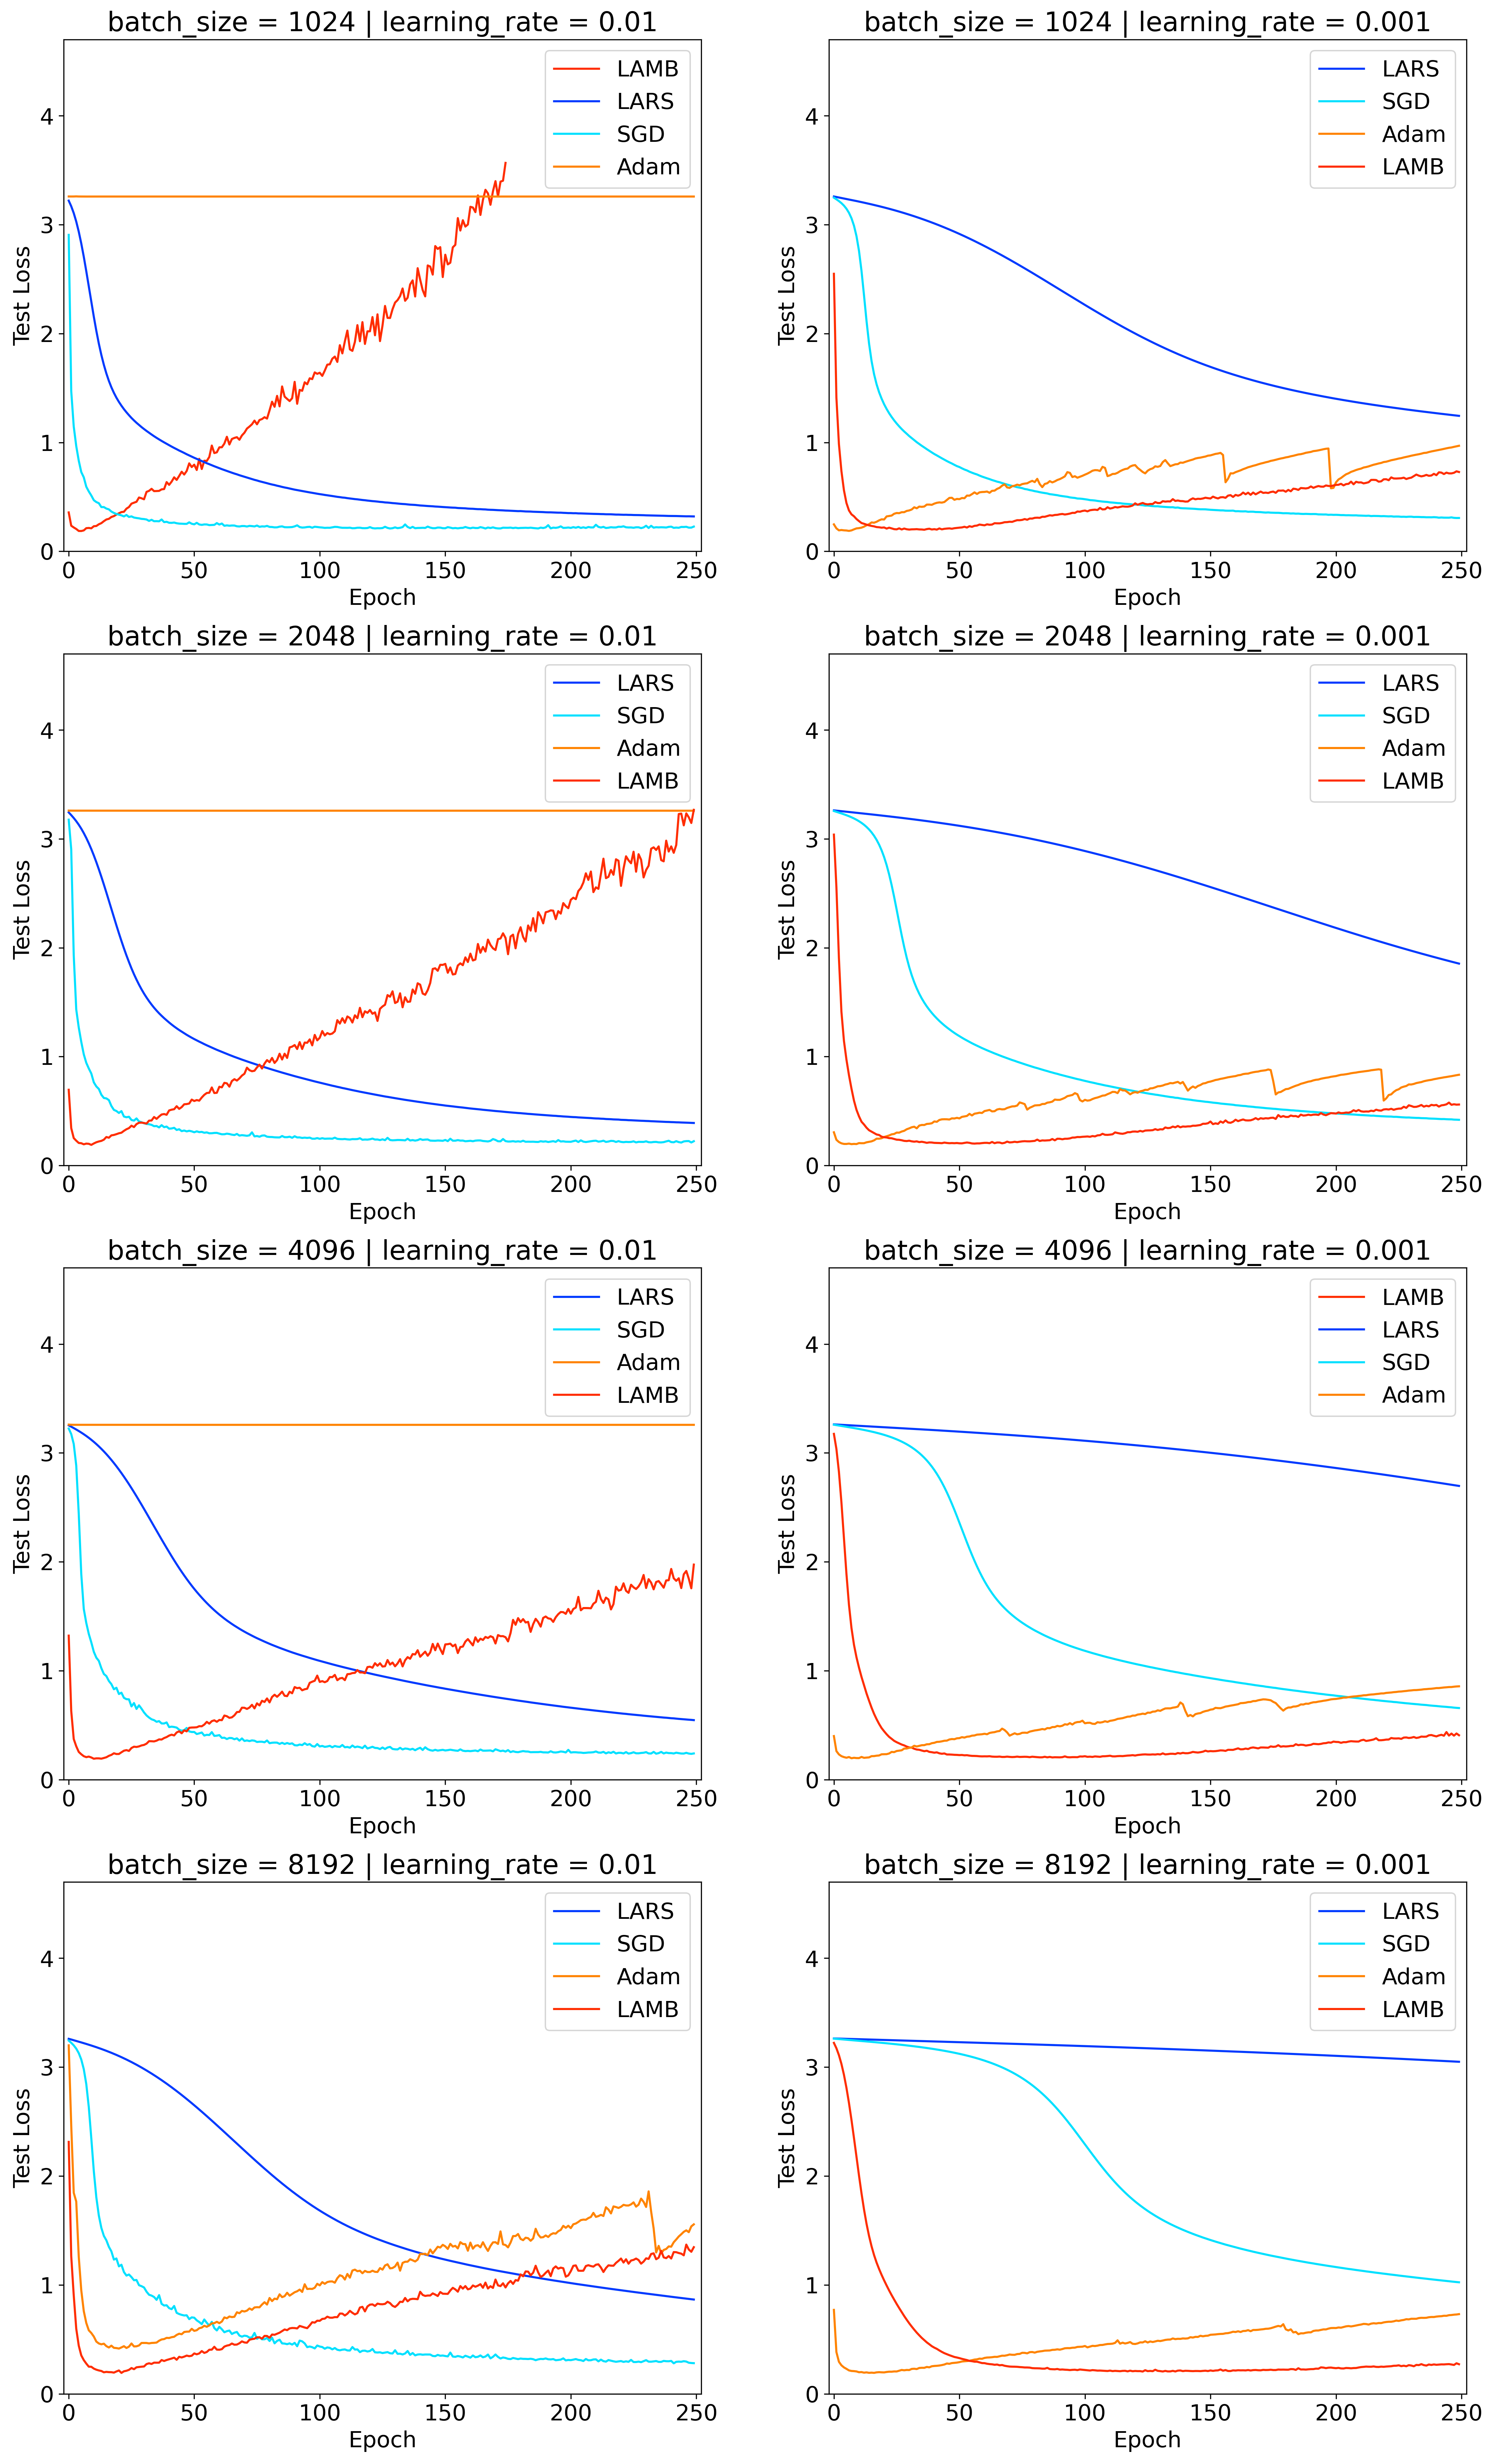
\includegraphics[width=0.7\linewidth, height=0.7\textheight]{img/eminst_all_figures.png}
    \caption{Image Classification test loss convergence rate during training based on optimizers (SGD, Adam, LARS, LAMB) across different batch sizes (1024, 2056, 4096, 8192) for learning rate of 0.01 (left plots) and 0.001 (right plots). }
    \label{fig:cv_plots}
\end{figure*}

\subsubsection{Evaluation}

The model's loss function for updating each batch and epoch is the sum of cross entropy between the predicted and actual of the two tokens. 


\subsection{Speech-to-Text Setup}


% SpeechRecognitionModel(
%   (cnn): Conv2d(1, 32, kernel_size=(3, 3), stride=(2, 2), padding=(1, 1))
%   (rescnn_layers): Sequential(
%     (0): ResidualCNN(
%       (cnn1): Conv2d(32, 32, kernel_size=(3, 3), stride=(1, 1), padding=(1, 1))
%       (cnn2): Conv2d(32, 32, kernel_size=(3, 3), stride=(1, 1), padding=(1, 1))
%       (dropout1): Dropout(p=0.3, inplace=False)
%       (dropout2): Dropout(p=0.3, inplace=False)
%       (layer_norm1): CNNLayerNorm(
%         (layer_norm): LayerNorm((64,), eps=1e-05, elementwise_affine=True)
%       )
%       (layer_norm2): CNNLayerNorm(
%         (layer_norm): LayerNorm((64,), eps=1e-05, elementwise_affine=True)
%       )
%     )
%     (1): ResidualCNN(
%       (cnn1): Conv2d(32, 32, kernel_size=(3, 3), stride=(1, 1), padding=(1, 1))
%       (cnn2): Conv2d(32, 32, kernel_size=(3, 3), stride=(1, 1), padding=(1, 1))
%       (dropout1): Dropout(p=0.3, inplace=False)
%       (dropout2): Dropout(p=0.3, inplace=False)
%       (layer_norm1): CNNLayerNorm(
%         (layer_norm): LayerNorm((64,), eps=1e-05, elementwise_affine=True)
%       )
%       (layer_norm2): CNNLayerNorm(
%         (layer_norm): LayerNorm((64,), eps=1e-05, elementwise_affine=True)
%       )
%     )
%     (2): ResidualCNN(
%       (cnn1): Conv2d(32, 32, kernel_size=(3, 3), stride=(1, 1), padding=(1, 1))
%       (cnn2): Conv2d(32, 32, kernel_size=(3, 3), stride=(1, 1), padding=(1, 1))
%       (dropout1): Dropout(p=0.3, inplace=False)
%       (dropout2): Dropout(p=0.3, inplace=False)
%       (layer_norm1): CNNLayerNorm(
%         (layer_norm): LayerNorm((64,), eps=1e-05, elementwise_affine=True)
%       )
%       (layer_norm2): CNNLayerNorm(
%         (layer_norm): LayerNorm((64,), eps=1e-05, elementwise_affine=True)
%       )
%     )
%   )
%   (fully_connected): Linear(in_features=2048, out_features=500, bias=True)
%   (birnn_layers): Sequential(
%     (0): BidirectionalGRU(
%       (BiGRU): GRU(500, 500, batch_first=True, bidirectional=True)
%       (layer_norm): LayerNorm((500,), eps=1e-05, elementwise_affine=True)
%       (dropout): Dropout(p=0.3, inplace=False)
%     )
%     (1): BidirectionalGRU(
%       (BiGRU): GRU(1000, 500, bidirectional=True)
%       (layer_norm): LayerNorm((1000,), eps=1e-05, elementwise_affine=True)
%       (dropout): Dropout(p=0.3, inplace=False)
%     )
%     (2): BidirectionalGRU(
%       (BiGRU): GRU(1000, 500, bidirectional=True)
%       (layer_norm): LayerNorm((1000,), eps=1e-05, elementwise_affine=True)
%       (dropout): Dropout(p=0.3, inplace=False)
%     )
%   )
%   (classifier): Sequential(
%     (0): Linear(in_features=1000, out_features=500, bias=True)
%     (1): GELU()
%     (2): Dropout(p=0.3, inplace=False)
%     (3): Linear(in_features=500, out_features=29, bias=True)
%   )
% )
% image of the network is the network.png
% https://www.assemblyai.com/blog/end-to-end-speech-recognition-pytorch




\subsubsection{Dataset}

The data was adopted from LibriSpeech \cite{7178964} which are audio recordings of public domain audio books of 100 hours for training and 5 hours for testing. It was preprocessed into spectrograms at a sample rate of 16khz. The task is to map an audio spectrogram frame to one of the 29 output classes (26 alphabet characters, an apostrophe, a space, and an <END> token). 


\subsubsection{Implementation Details}

Residual CNN block includes: 3 layers with 32x32 window size, stride of 2. A fully connected layer from ResCNN to GRU-RNN with 2048 to 500 dimension. Bidirectional GRU-RNN block have three layers with 500 input feature dim and 1000 output features. A final fully connected layer with 1000 input and 500 output. Dropout of 30\%.


\subsubsection{Evaluation}

The model is trained on the Connectionist Temporal Classification (CTC) loss function when aligning audio to transcript, which was originated by Graves et al. \cite{CTC} as shown here for a single (X, Y) pair: 
\begin{center}
$p(Y | X) = \sum_{A\in A_{X, Y}} \prod_t^T = p_t(a_t |. X)$    
\end{center}

CTC first computed the probability for a single alignment step-by-step over multiple sequences then marginalizes over the set of valid alignments to get a distribution over outputs.  
% at least 2-2.5 pages

% different subsections for each subsection type (NLP, computer vision, speech processing)

% for each section, start with the initial model, mention/explain the metrics used to evaluate (so overall accuracy or F1 score, etc basically anything logged in tensorboard)
% definitely mention the loss function used (binary cross entropy etc.)

% final section will mention the metrics we are saving for the adam/lamb, sgd/lars and how we will compare them (using tensoboard logs while running with similar input params (such as the learning rate / beta / eps))

% \section{Results}
% \label{sec:results}
% \subsection{Image Classification}
% lf 0.01

% Sgd & 0.20985 & 0.21054 & 0.23648 & 0.27958 & \\
% Lars & 0.32058 & 0.39033 & 0.54637 & 0.86530 & \\
% Adam & 3.25820 & 3.25817 & 3.25811 & 0.41513 & \\
% Lamb & 0.18673 & 0.18932 & 0.19189 & 0.19151 & \\

% 0.001
% Sgd & 0.30633 & 0.41941 & 0.65746 & 1.02366 & \\
% Lars & 1.24437 & 1.85403 & 2.69716 & 3.04892 & \\
% Adam & 0.18780 & 0.19604 & 0.19640 & 0.19186 & \\
% Lamb & 0.19837 & 0.20102 & 0.20386 & 0.20411 & \\

\begin{table}[!t]
\vspace{-5pt}
\small
\vspace{7pt}
\caption{Image classification performance based on optimizers (SGD, Adam, LARS, LAMB) across different batch sizes (1024, 2048, 4096, 8192). Highlighted gray cells indicate best performing optimizer. The learning rate of the top and bottom table are 0.01 and 0.001 respectively.}\label{tbl:img_results}
\vspace{-10pt}
\begin{center}
\begin{tabular}{ c|c|c|c|c}
\multicolumn{1}{c|}{} &  \multicolumn{4}{c}{Batch Size}\\ \cline{2-5}
\multicolumn{1}{c|}{Optimizer} &
 \multicolumn{1}{c|}{1024} &
 \multicolumn{1}{c|}{2048} &
 \multicolumn{1}{c|}{4096} &
 \multicolumn{1}{c}{8192} \\
 \hline
SGD & 0.21 & 0.21 & 0.24 & 0.28 \\
LARS & 0.32 & 0.39 & 0.55 & 0.87 \\
Adam & 3.26 & 3.26 & 3.26 & 0.42 \\
LAMB & \cellcolor{gray!30} 0.19 & \cellcolor{gray!30} 0.19 & \cellcolor{gray!30} 0.19 & \cellcolor{gray!30}  0.19 \\

\end{tabular}

\vspace{10pt}

%%%%%%%%%%%%%%%%%%%%%%%%%%%%%%%%%%%%%%%%%%%%%%%%%%%%%%%%%%%%%%%%%%%%%
\begin{tabular}{ c|c|c|c|c}
\multicolumn{1}{c|}{} &  \multicolumn{4}{c}{Batch Size}\\ \cline{2-5}
\multicolumn{1}{c|}{Optimizer} &
 \multicolumn{1}{c|}{1024} &
 \multicolumn{1}{c|}{2048} &
 \multicolumn{1}{c|}{4096} &
 \multicolumn{1}{c}{8192} \\ \hline
SGD & 0.31 & 0.42 & 0.66 & 1.02 \\
LARS & 1.24 & 1.85 & 2.70 & 3.05 \\
Adam & \cellcolor{gray!30} 0.19 & \cellcolor{gray!30} 0.20 & \cellcolor{gray!30} 0.20 & \cellcolor{gray!30} 0.19 \\
LAMB & 0.20 & \cellcolor{gray!30} 0.20 & \cellcolor{gray!30} 0.20 & 0.20 \\

\end{tabular}
\vspace{-15pt}
\end{center}
\end{table}

The result of image classification is shown in Table \ref{t}. We researched four optimizers (SGD, Adam, LARS, LAMB) across four different batch sizes (1024, 2048, 4096, 8192) with two different learning rate (0.01, 0.001). 


\subsection{QA System}

\begin{table}[!t]
\vspace{-5pt}
\small
\vspace{7pt}
\caption{QA System performance based on optimizers (SGD, Adam, LARS, LAMB) across different batch sizes (64, 128, 256, 512). Highlighted gray cells indicate best performing optimizer.}\label{tbl:qa_results}
\vspace{-10pt}
\begin{center}
\begin{tabular}{ c|c|c|c|c}
\multicolumn{1}{c|}{} &  \multicolumn{4}{c}{Batch Size}\\ \cline{2-5}
\multicolumn{1}{c|}{Optimizer} &
 \multicolumn{1}{c|}{64} &
 \multicolumn{1}{c|}{128} &
 \multicolumn{1}{c|}{256} &
 \multicolumn{1}{c}{512} \\
 %& & \\
\hline
SGD & 4.76 & 5.00 & 5.38 & 6.45\\
Adam &  4.59 & \cellcolor{gray!30} 4.59 &  \cellcolor{gray!30} 4.49 & \cellcolor{gray!30} 4.53\\
LARS & 8.36 & 8.42 & 8.57 & 9.43\\
LAMB & \cellcolor{gray!30} 4.58 & 4.62 & 4.59 & 4.86\\
\end{tabular}
\end{center}
\vspace{-15pt}
\end{table}



\begin{figure}[!t]
    \centering
    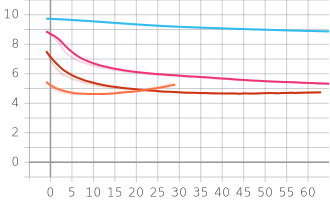
\includegraphics[width=0.7\linewidth]{img/drqa_128_blars_oadam_psgd_rlamb.png}
    \caption{LARS (light blue), SGD (pink), LAMB (red), and Adam (orange) test loss convergence graph.}
    \label{fig:128}
\end{figure}

The experimentation is conducted by deploying the model from \S\ref{sec:method}.B against the dedicated four optimizers in this study (SGD, Adam, LARS, and LAMB) across various batch sizes (64, 128, 256, 512). The results are reported in the Table~\ref{tbl:qasystem}. The gray cells denote the winner (the one with the lowest loss overall test loss values in the same column) across each batch size. The results were surprising as LAMB only outperformed Adam in a batch size of 64 but lost in the other batch sizes. LARS performed the worst across every run, where it was bested by traditional SGD consistently. Moreover, as the batch size increased, the gap between performances increased. This contradicts what has been observed in current literature \cite{ginsburg2018large}. We did not observe the performance increase of the QA system with larger batch sizes across the layer-wise adaptive techniques. However, there are two possible explanations for these results, which include: 
\begin{itemize}
    \item The batch sizes tested in the QA system were statistically small in comparison to most literature (which reported sizes of 4K or >8K)
    \item Based on Figure \ref{fig:256}, Adam over-fitted a lot more quickly and triggered the early stop procedure, while the other algorithms did not. A similar trend can be observed in Figure \ref{fig:128} where LAMB converged very slowly and it can easily be deduced that a longer training time would allow for an even lower test loss value (and higher overall accuracy) than ADAM ever could reach
\end{itemize}

\subsection{Speech-to-Text}
\begin{table}[!t]
\vspace{-5pt}
\small
\vspace{7pt}
\caption{Speech-to-Text performance based on optimizers (SGD, Adam, LARS, LAMB) across different batch sizes (8, 16, 32). Highlighted gray cells indicate best performing optimizer.}\label{tbl:speech_results}
\vspace{-10pt}
\begin{center}
\begin{tabular}{ c|c|c|c}
 &  \multicolumn{3}{c}{Batch Size}\\ 
\cline{2-4}
\multicolumn{1}{c|}{Optimizer} &
 \multicolumn{1}{c|}{8} &
 \multicolumn{1}{c|}{16} &
 \multicolumn{1}{c}{32}  \\
\hline
SGD & 2.80 & 2.83 & 2.85 \\
LARS & NaN* & NaN* & 2.86 \\
Adam & \cellcolor{gray!30} 1.03 & 2.21 & \cellcolor{gray!30}  0.77 \\
LAMB & 1.06 & \cellcolor{gray!30} 0.89 & 1.17 \\
\end{tabular}
\end{center}
\vspace{-15pt}
\end{table}
% 2 pages

% put graphs for at least one of each of the models tested (overlay the data from the proper comparison)

% \section{Threats of Validity}
% \label{sec:threats}
% \subsection{Evaluation Bias}

This paper employed the accuracy for image classification loss, perplexity for question answering, and text to speech. There are other evaluation scores that could be applied to this kind of analysis
and, in the future, it would be useful to test in the central claim of this paper holds for more than the aforementioned ones.

\subsection{Learner Bias}

This study utilized LSTMs layers for question answering system, CNN for image classifications, and ResNet for speech to text task. 
The case was made in \S4.4 that this represents an interesting range of current problem domains.
Nevertheless, it might be useful in future work to test if the central claim of this paper 
hold across multiple up-to-date models (e.g. transformers) across several domains.

\subsection{Sampling Bias}

Like any data mining paper,
our work is threatened by sampling bias; i.e. what holds for the data we studied here may
not hold for other kinds of data. 
Within the space of one paper, it is hard to avoid sampling bias.
However, what researchers can do is make all their scripts and data available
such that other researchers can test their conclusions whenever new data becomes available. To that end, we have made all our scripts and data available at github.com/HuyTu7/dl\_optimizers.
% .5 pages



% \section{Conclusion and Future Work}
% \label{sec:conclusion}
% This paper have investigated the effectiveness of LARS and LAMB across multiple machine learning domains (NLP, CV, and Speech), model sizes (a median of 13 million parameters), and batch sizes (8 - 8K) to find that:  

\begin{enumerate}
    \item The results of You et al. is reproducible and validated through  one of the initial domains tested by You et al.  \cite{You2020Large} (image classification in section V.A). Yet, LARS surprisingly underperformed SGD even with large batch sizes.
    \item Layer-wise optimization techniques (LARS and LAMB) on smaller batch sizes training do not work as well as traditional optimizers (Adam and SGD). 
\end{enumerate}

However, there are two possible explanations for the negative results of the layer-wise optimizers (LAMB and LARS) on the two case studies performed in the scope of this paper (QA System and Speech to Text), which include: 
\begin{itemize}
    \item The batch sizes tested in the QA system were statistically small in comparison to most literature (which reported sizes of 8K and up to 64K)
    \item Through the training plots (for QA System and Speech to Text), we observe that Adam over-fitted a lot more quickly (within 10 epochs) and triggered the early stop procedure, while the other algorithms did not. At the same time, LAMB converged very slowly and it can easily be deduced that a longer training time would allow for an even lower test loss value than ADAM ever could reach.
    \item The learning rate had a large effect on the overall performance of all the layer-wise adaptive models, and more testing should be performed across a range of learning rates to create a better control environment.
\end{itemize}


% .5 pages

\balance
\bibliographystyle{IEEEtranN}
\bibliography{bibliography.bib}



\end{document}